\documentclass[10pt]{article}
\usepackage{parskip}
\usepackage[utf8]{inputenc}
\usepackage[left=2.00cm, right=2.00cm, top=2.00cm, bottom=2.00cm]{geometry}
\usepackage[spanish]{babel}
\usepackage{graphicx,subfig}
\usepackage{fancyhdr}
\usepackage{pgfplots}
\graphicspath{{Imagenes/}}
\usepackage{enumerate} 
\usepackage{multicol}
\usepackage{tabularx}
\usepackage{amssymb}
\usepackage{adjustbox}
\usepackage{amsmath}
\usepackage{cancel}
\begin{document}


\pagestyle{fancy}
\cfoot{}


%Cabeceras
\rhead{Ley de Ohm.}
\lhead{}

%Portada
\begin{titlepage}
	\newgeometry{
		left=25mm,
		right=25mm,
		top=5mm,
		bottom=30mm,
		headheight = 0 mm
	}

	\begin{figure}[t]
		\subfloat{
\includegraphics[width=0.15\textwidth]{Logo_IPN}}
		\hspace{0.6\textwidth}
		\subfloat{
\includegraphics[width=0.22\textwidth]{LogoEsime}}
	\end{figure}

	\centering
	{\bfseries\Huge Instituto Politécnico Nacional. \par}
	\vspace{1cm}
	{\scshape\Large Ingeniería en Comunicaciones y Electrónica. \par}
	\vspace{0.3cm}
	{\scshape\Large Laboratorio de Electricidad y Magnetismo.  \par}
	\vspace{1cm}
	{\scshape\Huge Victoria la Reina Insaciable \par}
	\vspace{1cm}
	{\itshape\Large Ley de Ohm. \par}
	{\Large 2CM13\par}
	\vfill
	{\Large Autores: \par}
	{\Large Daniela Elizabeth Pérez Vargas. \par}
	{\Large Jesús Martinez Amac. \par}
	{\Large José Emilio Hernández Huerta. \par}
	{\Large Nataly Bejarano Garduño.\par}
	{\Large Uriel Grimaldi Díaz.  \par}
	\vfill
	{\Large Junio 2023. \par}

\end{titlepage}

\tableofcontents
\newpage

\section{Resumen.}
En la practica con el material especifico comprobamos la ley de ohm midiendo desde el potencial electrico como la intensidad mediante un circuito en serie el cual regulamos con una caja especial con la cual podemos variar la recistencia que esta experimenta y tambien con un switch integrado en el circuito para hacer más facil el cambio en la funte de alimentacion terminando con la tabulacion de los resultados. 

\begin{multicols}{2}

\section{Objetivo.}
Se verificara que la corriente en un resistor ohmico es directamente proporcional a la diferencia de potencial entre sus bornes, dentro de los limites de precision del experimento, tambien establecera la relacion matematica entre la resistencia de un resistor ohmico y la corriente que lo atraviesa cuando el voltaje permanece constante y vericaran el comportamiento del circuito al variar la resistencia y el voltaje para mantener la corriente constante.


\section{Introducción.}
En nuestra formacion como ingenieros electronicos necesitaremos las bases para comprender, analizar, crear, reparar y entre muchos más, sistemsas electronicos pero para esto es sumamnete necesaria la ley de Ohm la cual establece que la diferencia de potencial que aplicamos entre los extremos de un conductor determinado es proporcional a la intensidad de la corriente que circula por el citado conductor.
Aunque esto parezca innecesario las practicas de laboratorio son importantes pues como en la vida laborar si aqui nos equivocamos quemando algun material tendremos consecuencia pero mientras que afuera seria un despido aqui solo es reponer el material y en tu calificacion, asi que le doy animos a cualquiera que lea este reporte.


\section{Marco teórico.}

La ley de Ohm establece una relación directa y proporcionalidad entre la corriente eléctrica y la diferencia de potencial (voltaje) en un circuito eléctrico cerrado (1)(2). En su forma más básica, la ley de Ohm establece que la corriente que fluye a través de un conductor es igual a la diferencia de voltaje entre los extremos del mismo (2)(3) , dividida por la resistencia del conductor:
$I = V/R$
Donde I es la corriente en amperios, V es la diferencia de voltaje en voltios (3) y R es la resistencia eléctrica del conductor en ohmios. Por lo tanto, la corriente y el voltaje están estrechamente relacionados en un circuito eléctrico. Además, la ley de Ohm también puede usarse para calcular la resistencia eléctrica de un conductor (2) diferencia de voltaje necesaria para producir una corriente determinada (3) o la corriente que fluirá en un circuito de resistencia determinada a partir de una diferencia de voltaje conocida.
\begin{center}
	
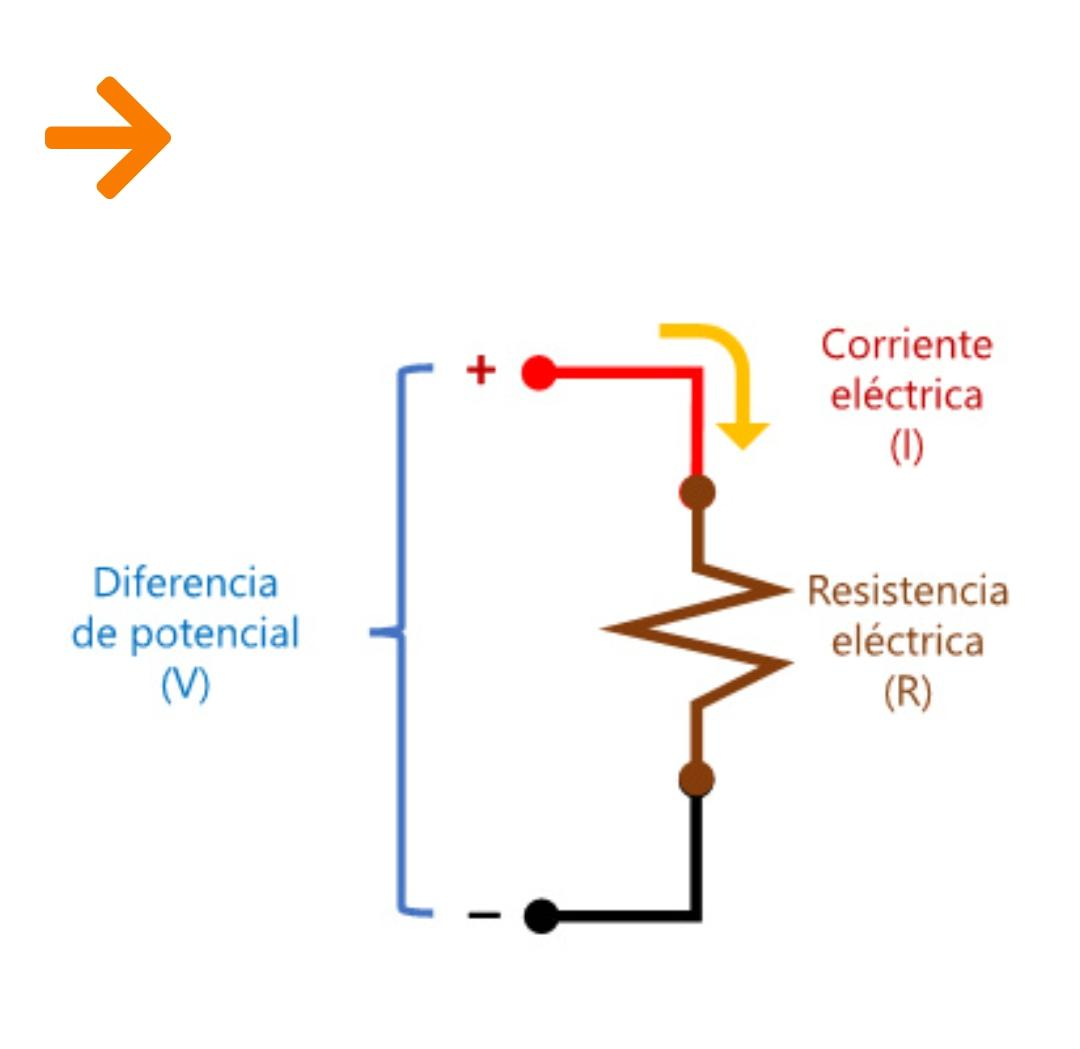
\includegraphics[width=0.17\textwidth]{lol}\\
Circuito Electrico \newline
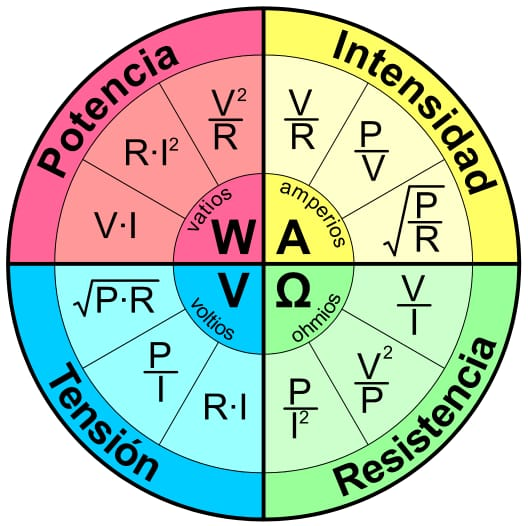
\includegraphics[width=0.17\textwidth]{reina}\\
Formulas para ley de Ohm

\end{center}
\section{Descripción de materiales.}



\section{Desarrollo experimental.}

1.-Relación entre voltaje y corriente. 
En este primer ejercicio se requirió armar un circuito teniendo precaución de que el selector del medidor este señalado la escala de 3 mA  o mayor y que la escala de voltaje de la fuente no marque más de 15 volts. 
Posterior a esto y después de comprobar que el circuito estaba bien armado, cerramos el interruptor K y con los controles (grueso y fino) de salida de voltaje de la fuente regulada ajustamos el voltaje de acuerdo a los valores indicados en la tabla.
 
2.- Relación entre resistencia y corriente. 
Con el circuito posteriormente armado encendimos la fuente regulada y con ayuda de los controles (grueso y fino) ajustamos el voltaje de salida aplicado al resistor a un valor de 8 volts. 
Realizando lo anterior cerramos el interruptor K y medimos la intensidad de corriente para cada valor de resistencia, (abriendo el interruptor K antes del cambio de resistencia). 

3.- Relación entre voltaje y resistencia 
Con el mismo circuito cerramos el interruptor K y lentamente con ayuda de los controles aumentamos el voltaje aplicando a la resistencia hasta que el amperímetro se obtenga una lectura de 2 Ma, cuando alcanzamos este valor (abrimos el interruptor K incrementando el valor de la resistencia según lo indicado en la tabla



\section{Analisis de resultados}




\begin{center}
	\begin{adjustbox}{width=245pt}
		\begin{tabular}{|c|c|c|c|c|}
			\hline
			Resistencia & Colores & Tolerancia & Valor nominal (ohms) & Valor medido (ohms) \\
			\hline
			1 & Café, verde, rojo, dorado & $\pm$ 5\% & 1.5k & 1.46k \\
			\hline
			2 & Rojo, azul, rojo, dorado & $\pm$ 5\% & 2.6k & 2.18k \\
			\hline
			3 & Naranja, naranja, naranja, dorado & $\pm$ 5\% & 33k & 32.8k \\
			\hline
			4 & Amarillo, violeta, rojo, dorado & $\pm$ 5\% & 4.7k & 4.75k \\
			\hline
			5 & Azul, verde, rojo, dorado & $\pm$ 5\% & 6.5k & 6.66k \\
			\hline
		\end{tabular}
	\end{adjustbox}
\end{center}


\section{Conclusiones.}

\subsection*{José Emilio Hernández Huerta.}
Durante la práctica, pude verificar que la corriente es directamente proporcional a la tensión aplicada y que disminuye cuando se incrementa la resistencia. Esto me ha enseñado la importancia de elegir los componentes adecuados para garantizar un funcionamiento óptimo del circuito, así como la necesidad de considerar la resistencia al diseñar y analizar circuitos eléctricos. 

\subsection*{Daniela Elizabeth Pérez Vargas.}
En conclusión, la Ley de Ohm establece una relación directa entre la intensidad de corriente que fluye a través de un resistor y la diferencia de potencial aplicada a sus terminales. Esta ley es fundamental para el estudio de la electricidad y es aplicable en una gran variedad de circuitos eléctricos. Asimismo, la ley de Ohm es importante en la resolución de problemas de circuitos eléctricos en la vida real y en el diseño de sistemas eléctricos más eficientes. A través de la experimentación y el análisis de las magnitudes eléctricas.
\subsection*{Jesús Martinez Amac.}

\subsection*{Nataly Bejarano Garduño.}
El “voltaje” o Diferencial de potencial eléctrico, es el trabajo por unidad de carga eléctrica que ejerce sobre una partícula un campo eléctrico. La resistencia es una medida de la oposición al flujo de corriente en un circuito eléctrico La corriente eléctrica es el flujo de carga eléctrica que atraviesa un material conductor durante un periodo de tiempo determinado. 
La relación entre corriente, voltaje y resistencia se expresa por la ley de Ohn. Determina que la corriente que fluye en un circuito es proporcionar directamente al voltaje aplicado e inversamente proporcional a la resistencia del circuito, y aunque son parecidas no son lo mismo, aunque si se complementan.

\subsection*{Uriel Grimaldi Díaz.}


\begin{thebibliography}{0}
	\bibitem{citekey}[Ley de Ohm . (2021, 1 de marzo). Portal Académico Del CCH.]
	\bibitem{citekey}[La ley de Ohm - Electricidad y electrónica - Picuino . (Dakota del Norte)]
		
\end{thebibliography}

\end{multicols}

\end{document}
